\pdfminorversion=4
\documentclass{beamer}

\usepackage[toc]{beamerthemecea2019}
\usepackage[T1]{fontenc}
\usepackage[utf8]{inputenc}

\usepackage{longtable}
%\usepackage{couleurs}
\usepackage{listings}
%\usepackage{mecanique}
\usepackage{pifont}% http://ctan.org/pkg/pifont
\usepackage{animate,subcaption}

\newcommand{\dx}{\text{ dx}}
\newcommand{\dS}{\text{ dS}}
\newcommand{\udl}[1]{\boldsymbol{#1}}
\newcommand{\uddl}[1]{\boldsymbol{#1}}
\renewcommand{\div}{\operatorname{div}}
\newcommand{\bg}{\boldsymbol{g}}
\newcommand{\bj}{\boldsymbol{j}}
\newcommand{\bu}{\boldsymbol{u}}
\newcommand{\bv}{\boldsymbol{v}}
\newcommand{\bvarepsilon}{\boldsymbol{\varepsilon}}
\newcommand{\bsig}{\boldsymbol{\sigma}}
\newcommand{\bD}{\boldsymbol{D}}
\newcommand{\bE}{\boldsymbol{E}}
\newcommand{\bF}{\boldsymbol{F}}
\newcommand{\bR}{\boldsymbol{R}}
\newcommand{\bH}{\boldsymbol{H}}
\newcommand{\bI}{\boldsymbol{I}}
\newcommand{\bP}{\boldsymbol{P}}
\newcommand{\bS}{\boldsymbol{S}}
\newcommand{\bT}{\boldsymbol{T}}
\newcommand{\bV}{\boldsymbol{V}}
\newcommand{\bY}{\boldsymbol{Y}}
\newcommand{\Bb}{\mathcal{B}}
\newcommand{\Dd}{\mathcal{D}}
\newcommand{\Ee}{\mathcal{E}}
\newcommand{\CC}{\mathbb{C}}
\newcommand{\DD}{\mathbb{D}}
\newcommand{\TT}{\mathbb{T}}
\newcommand{\Sig}{\boldsymbol{\Sigma}}
\newcommand{\T}{^\text{T}}
\newcommand{\jump}[1]{[\![#1]\!]}
\DeclareMathOperator*{\argmin}{arg\,min}
\DeclareMathOperator{\tr}{tr}
\newcommand{\pavg}[1]{\left\langle #1 \right\rangle}

\newcommand{\Cxx}{\texttt{C\nolinebreak\hspace{-.05em}\raisebox{.4ex}{\tiny\bf +}\nolinebreak\hspace{-.10em}\raisebox{.4ex}{\tiny\bf +}}
  \def\CC{{C\nolinebreak[4]\hspace{-.05em}\raisebox{.4ex}{\tiny\bf ++}}}}
\newcommand{\tfel}{\href{http://www.tfel.sourceforge.net}{\texttt{TFEL}}}
\newcommand{\mfront}{\href{http://www.tfel.sourceforge.net}{\texttt{MFront}}}
\newcommand{\cea}{\href{http://www.cea.fr}{CEA}}
\newcommand{\edf}{\href{http://www.edf.com}{EDF}}
\newcommand{\inria}{\href{http://www.inria.fr}{INRIA}}
\newcommand{\gcc}{\href{https://gcc.gnu.org/}{gcc}}
\newcommand{\clang}{\href{clang.llvm.org}{clang}}
\newcommand{\icc}{\href{https://software.intel.com/en-us/c-compilers}{icc}}
\newcommand{\msys}{\href{http://www.mingw.org/wiki/MSYS}{MSYS}}
\newcommand{\jenkins}{\href{http://jenkins-ci.org}{\texttt{Jenkins}}}
\newcommand{\gpl}{\href{http://www.gnu.org/licenses/gpl-3.0.txt}{GNU Public License}}
\newcommand{\unix}{\texttt{Unix}}
\newcommand{\linux}{\texttt{LiNuX}}
\newcommand{\freebsd}{\href{https://www.freebsd.org/}{\texttt{FreeBSD}}}
\newcommand{\opensolaris}{\texttt{OpenSolaris}}
\newcommand{\cygwin}{\texttt{cygwin}}
\newcommand{\wsl}{\texttt{Windows Subsystem for LiNuX}}
\newcommand{\haiku}{\texttt{Haiku}}
\newcommand{\mtest}{\texttt{mtest}}
\newcommand{\absvalue}[1]{{\left|#1\right|}}

\usepackage{fancyvrb}
\providecommand{\tightlist}{%
  \setlength{\itemsep}{0pt}\setlength{\parskip}{0pt}}
\newcommand{\VerbBar}{|}
\newcommand{\VERB}{\Verb[commandchars=\\\{\}]}
\DefineVerbatimEnvironment{Highlighting}{Verbatim}{commandchars=\\\{\}}
\newenvironment{Shaded}{}{}
\newcommand{\AlertTok}[1]{\textcolor[rgb]{1.00,0.00,0.00}{\textbf{#1}}}
\newcommand{\AnnotationTok}[1]{\textcolor[rgb]{0.38,0.63,0.69}{\textbf{\textit{#1}}}}
\newcommand{\AttributeTok}[1]{\textcolor[rgb]{0.49,0.56,0.16}{#1}}
\newcommand{\BaseNTok}[1]{\textcolor[rgb]{0.25,0.63,0.44}{#1}}
\newcommand{\BuiltInTok}[1]{#1}
\newcommand{\CharTok}[1]{\textcolor[rgb]{0.25,0.44,0.63}{#1}}
\newcommand{\CommentTok}[1]{\textcolor[rgb]{0.38,0.63,0.69}{\textit{#1}}}
\newcommand{\CommentVarTok}[1]{\textcolor[rgb]{0.38,0.63,0.69}{\textbf{\textit{#1}}}}
\newcommand{\ConstantTok}[1]{\textcolor[rgb]{0.53,0.00,0.00}{#1}}
\newcommand{\ControlFlowTok}[1]{\textcolor[rgb]{0.00,0.44,0.13}{\textbf{#1}}}
\newcommand{\DataTypeTok}[1]{\textcolor[rgb]{0.56,0.13,0.00}{#1}}
\newcommand{\DecValTok}[1]{\textcolor[rgb]{0.25,0.63,0.44}{#1}}
\newcommand{\DocumentationTok}[1]{\textcolor[rgb]{0.73,0.13,0.13}{\textit{#1}}}
\newcommand{\ErrorTok}[1]{\textcolor[rgb]{1.00,0.00,0.00}{\textbf{#1}}}
\newcommand{\ExtensionTok}[1]{#1}
\newcommand{\FloatTok}[1]{\textcolor[rgb]{0.25,0.63,0.44}{#1}}
\newcommand{\FunctionTok}[1]{\textcolor[rgb]{0.02,0.16,0.49}{#1}}
\newcommand{\ImportTok}[1]{#1}
\newcommand{\InformationTok}[1]{\textcolor[rgb]{0.38,0.63,0.69}{\textbf{\textit{#1}}}}
\newcommand{\KeywordTok}[1]{\textcolor[rgb]{0.00,0.44,0.13}{\textbf{#1}}}
\newcommand{\NormalTok}[1]{#1}
\newcommand{\OperatorTok}[1]{\textcolor[rgb]{0.40,0.40,0.40}{#1}}
\newcommand{\OtherTok}[1]{\textcolor[rgb]{0.00,0.44,0.13}{#1}}
\newcommand{\PreprocessorTok}[1]{\textcolor[rgb]{0.74,0.48,0.00}{#1}}
\newcommand{\RegionMarkerTok}[1]{#1}
\newcommand{\SpecialCharTok}[1]{\textcolor[rgb]{0.25,0.44,0.63}{#1}}
\newcommand{\SpecialStringTok}[1]{\textcolor[rgb]{0.73,0.40,0.53}{#1}}
\newcommand{\StringTok}[1]{\textcolor[rgb]{0.25,0.44,0.63}{#1}}
\newcommand{\VariableTok}[1]{\textcolor[rgb]{0.10,0.09,0.49}{#1}}
\newcommand{\VerbatimStringTok}[1]{\textcolor[rgb]{0.25,0.44,0.63}{#1}}
\newcommand{\WarningTok}[1]{\textcolor[rgb]{0.38,0.63,0.69}{\textbf{\textit{#1}}}}

% orange
\definecolor{lightorange}{rgb}{1.0,0.63921,0.3961}		
\definecolor{orange}{rgb}{1.0,0.5098, 0}		

% chocolate (brownish)
\definecolor{my_blue}{rgb}{0.09019,0.4706,1.0}
\definecolor{lightblue}{rgb}{0.8588,0.9490,1.0}


\newcommand{\cmark}{\textcolor{green}{\ding{51}}}%
\newcommand{\xmark}{\textcolor{red}{\ding{55}}}%


\lstset{ %
  backgroundcolor=\color{white},   % choose the background color; you must add \usepackage{color} or \usepackage{xcolor}
  basicstyle=\tiny,       % the size of the fonts that are used for the code
  breakatwhitespace=false,         % sets if automatic breaks should only happen at whitespace
  breaklines=true,                 % sets automatic line breaking
  captionpos=b,                    % sets the caption-position to bottom
  commentstyle=\color{red},        % comment style
  deletekeywords={...},            % if you want to delete keywords from the given language
  frame=single,                    % adds a frame around the code
  keepspaces=true,                 % keeps spaces in text, useful for keeping indentation of code (possibly needs columns=flexible)
  keywordstyle=\color{blue},       % keyword style
  language=C++,                    % the language of the code
  morekeywords={Output Author Input Date},            % if you want to add more keywords to the set
  numbers=none,                    % where to put the line-numbers; possible values are (none, left, right)
  rulecolor=\color{orange},         % if not set, the frame-color may be changed on line-breaks within not-black text (e.g. comments (green here))
  showspaces=false,                % show spaces everywhere adding particular underscores; it overrides 'showstringspaces'
  showstringspaces=false,          % underline spaces within strings only
  showtabs=false,                  % show tabs within strings adding particular underscores
  stepnumber=1,                    % the step between two line-numbers. If it's 1, each line will be numbered
  stringstyle=\color{green},       % string literal style
  tabsize=8,                       % sets default tabsize to 2 spaces
  columns=flexible
}

\titre{\texttt{MFEM-MGIS}: an \texttt{MFEM}
  based application for non linear solid thermomechanics}
\evenement{MFEM Workshop} \date{10/2021}% \auteurprincipal{T. Helfer}
\auteurs{T. Helfer, G. Latu}

\newcommand{\gallery}[4]{
  \Titre{#1}
  \begin{frame}
    \begin{center}
      \includegraphics[width=#4\textwidth]{img/#2}
    \end{center}
    #3
  \end{frame}
}

\begin{document}

\PageTitre{}

\Titre{Outline}
\begin{frame}[fragile]
  \begin{flushleft}
    {\tiny
      \tableofcontents[hideallsubsections]      
    }
  \end{flushleft}
\end{frame}

\section{Context and goals}
\Intercalaire{Context and goals}

\Titre{The Pleiades platform}
\begin{frame}[fragile]
  \begin{center}
    \includegraphics[width=0.70\linewidth]{img/PLEIADES_2019_en.png}
  \end{center}
  \begin{itemize}
  \item A wide range of materials (ceramics, metals, composites).
  \item A wide range of mechanical phenomena and behaviours.
    \begin{itemize}
    \item Creep, swelling, irradiation effects, phase transitions, etc..
    \end{itemize}
  \item A wide range of mechanical loadings.
  \end{itemize}
\end{frame}

\Titre{Goals of MFEM-MGIS}
\frame{
  \begin{itemize}
    \item Build a HPC general purpose non linear multi-physics
    library
    \begin{itemize}
      \item Primary focus is non linear solid mechanics and
      heat transfer.
      \item Expected modelling: Shells, Beams, Phase-field
      approaches of brittle fracture, micromorphic models, Cosserat
      plasticity, strongly coupled thermo-chemical-mechanical or
      thermo-hydro-mechanical phenomena must also be considered.
    \end{itemize}
    \item  Two-pillar libraries:
    \begin{itemize}
      \item \texttt{MFEM}: HPC finite element solver.
      \item \texttt{MGIS/MFront}: constitutive laws, material modelling.
    \end{itemize}
  \end{itemize}
}

\section{A small tutorial}
\Intercalaire{A small tutorial}

\begin{frame}[fragile]{Final usage}
\protect\hypertarget{final-usage}{}
\vspace*{1mm}
{\tiny
\begin{Shaded}
\begin{Highlighting}[]
  \CommentTok{// loading the mesh}
  \KeywordTok{auto}\NormalTok{ mesh = }\BuiltInTok{std::}\NormalTok{make\_shared\textless{}mfem::Mesh\textgreater{}(mesh\_file, }\DecValTok{1}\NormalTok{, }\DecValTok{1}\NormalTok{);}
  \CommentTok{// building the non linear problem}
\NormalTok{  mfem\_mgis::NonLinearEvolutionProblem problem(}
      \BuiltInTok{std::}\NormalTok{make\_shared\textless{}mfem\_mgis::FiniteElementDiscretization\textgreater{}(}
\NormalTok{          mesh, }\BuiltInTok{std::}\NormalTok{make\_shared\textless{}mfem::H1\_FECollection\textgreater{}(order, dim), }\DecValTok{3}\NormalTok{),}
\NormalTok{      mgis::behaviour::Hypothesis::TRIDIMENSIONAL);}
  \CommentTok{// behaviour integrators}
\NormalTok{  problem.addBehaviourIntegrator(}\StringTok{"Mechanics"}\NormalTok{, }\DecValTok{1}\NormalTok{, library, behaviour);}
  \CommentTok{// materials}
  \KeywordTok{auto}\NormalTok{\& m1 = problem.getMaterial(}\DecValTok{1}\NormalTok{);}
\NormalTok{  mgis::behaviour::setExternalStateVariable(m1.s0, }\StringTok{"Temperature"}\NormalTok{, }\FloatTok{293.15}\NormalTok{);}
\NormalTok{  mgis::behaviour::setExternalStateVariable(m1.s1, }\StringTok{"Temperature"}\NormalTok{, }\FloatTok{293.15}\NormalTok{);}
  \CommentTok{// boundary conditions}
\NormalTok{  ...}
  \CommentTok{// solver parameters}
  \KeywordTok{auto}\NormalTok{\& solver = problem.getSolver();}
\NormalTok{  ...}
  \CommentTok{// loop over time step}
  \ControlFlowTok{for}\NormalTok{ (mfem\_mgis::}\DataTypeTok{size\_type}\NormalTok{ i = }\DecValTok{0}\NormalTok{; i != nsteps; ++i) \{}
    \CommentTok{// setting the boundary values}
\NormalTok{    ...}
    \CommentTok{// resolution}
\NormalTok{    problem.solve(dt);}
\NormalTok{    problem.update();}
\NormalTok{    t += dt;}
\NormalTok{  \}}
\end{Highlighting}
\end{Shaded}
}
\begin{itemize}
\tightlist
\item
  Straightforward to wrap in \texttt{python}.
\item
  Easy to integrate in a \texttt{PLEIADES} model (need
  \texttt{MEDCoupling} support)
\item
  The \texttt{NonLinearEvolutionProblem} class is the equivalent of
  \texttt{INCREPL}.
\item
  \textbf{Behaviour integrators} are the main new concept.
\end{itemize}
\end{frame}

\section{Design and features of the \texttt{MFEM-MGIS} project}
\Intercalaire{Design and features of the \texttt{MFEM-MGIS} project}

\Titre{MFront goals}
\begin{frame}
  \begin{center}
    \includegraphics[width=0.55\textwidth]{img/MFrontPrinciple.pdf}
  \end{center}
  \begin{itemize}
    \item {\tt MFront} is a code generation tool dedicated to
    material knowledge (material properties, mechanical behaviours,
    point-wise models):
    \begin{itemize}
      \item Support for small and finite strain behaviours,
      cohesive zone models, {\bf generalised behaviours} (non local and
      or multiphysics).
    \end{itemize}
    \item Main goals:
    \begin{itemize}
      \item Numerical efficiency (see various benchmarks on
      the website).
      \item Portability ({\tt Cast3M}, {\tt Cyrano}, {\tt
        code\_aster}, {\tt Europlexus}, {\tt TMFTT}, {\tt AMITEX\_FFTP},
      {\tt Abaqus}, {\tt CalculiX}, {\tt MTest}).
      \item {\bf Ease of use}: {\em Longum iter est per
        praecepta, breve et efficax per exempla} (It's a long way by the
      rules, but short and efficient with examples).
    \end{itemize}
  \end{itemize}
\end{frame}

\gallery{Modelling of abdominal muscles}{AbdominalMusclesModelling2019.png}{
  \begin{itemize}
    \item Hyperelastic behaviour in \texttt{code\_aster}
  \end{itemize}
}{0.9}

\gallery{Push-Pull on a concrete wall of concrete combined with heating}{FLBLITS.png}{
  \begin{itemize}
    \item Fichant-Laborderie damage behaviour coupled with LITS
    behaviour in \texttt{code\_aster}
    \item Comparison with experimental data (University of Buffalo, USA).
    \item Courtesy of J. Draup (EDF Energy, UK) and A. Gangnant
  \end{itemize}
}{0.9}

\gallery{Modelling of Drying schrinkage of wood with
  {\tt code\_aster} and {\tt MFront}}{WoodViscelasticity.jpg}{
  \begin{itemize}
    \item Club utilisateur {\tt MFront} 2020
    \item L. Riparbelli (University of Florence), I.
    Christovasilis (Aether Engineering), M. Fioravanti (University of
    Florence)
  \end{itemize}
}{0.5}

\gallery{Modélisation du freinage à partir d’une
  formulation thermomécanique avec {\tt code\_aster} et{\tt
    MFront}}{Braking.png}{
  \begin{itemize}
    \item Club utilisateur {\tt MFront} 2020
    \item - Thierry Ndzana Satoh (Université de Montpellier,
    SAFRAN Landing Systems), M. Renouf (Université de Montpellier), A.
    Chrysochoos (Université de Montpellier)
  \end{itemize}
}{0.7}

\gallery{Variational approaches to
  geomaterials}{Bacquaert.png}{
  \begin{itemize}
    \item Coupling damage and plasticity accounts for classical geomaterials behaviours (contractancy and dilatancy)
    \item Currently tested with the \texttt{mgis.fencis}
    `python` module. Shall be introduced in \texttt{code\_aster} during
    the PhD of G. Bacquaert.
    \item Courtesy of G. Bacquaert, V. Alves, Fernandes , J.
    Bleyer, D. Kondo, C. Maurini, S. Raude, F. Voldoire
  \end{itemize}
}{0.7}

\gallery{Polycrystal behaviour homogeneized by the
  Berveiller-Zaoui scheme}{BerveillerZaouiPolyCrystals.pdf}{
  \begin{itemize}
    \item Explicit (Runge-Kutta algorithm) and implicit
    implementation for a polycrystal of 240 grains (1453 internal state
    variables).
    \item The implicit scheme is original and unpublished yet.
    It shall be extended to abritrary complex single crytal behaviours
    and other homogeneisation schemes in 2021.
  \end{itemize}
}{0.5}

\gallery{Necking of a rod in finite strain plasticity}{mofem.pdf}{
  \begin{itemize}
    \item Example of usage of \texttt{MFront} in the
    \texttt{MoFEM} finite element solver.
    \item a) Discretised one eighth of the geometry. b)
    Parallel domain decomposition. c) Deformed specimen and distribution
    of deformation gradient.
    \item Courtesy of K. Lewandowski and L. Kaczmarczyk,
    University of Glasgow.
  \end{itemize}
}{0.7}

\gallery{Berkovich indentation on a single
  crystal}{Residual_imprint.png}{
  \begin{itemize}
    \item Normalised residual topography after an indentation
    test on a single crsytal of copper using \texttt{Ansys}
    \item Courtesy of A. Bourceret, FEMTO
    \item The implementation of the behaviour is described
    here: {\small \url{http://tfel.sourceforge.net/MericCailletaudSingleCrystalPlasticity.html}}
  \end{itemize}
}{0.45}

\gallery{Design of a cylinder
  block}{PSACylinderBlock.png}{
  \begin{itemize}
    \item Industrial thermomechanical design of a cylinder
    block with an with \texttt{MFront} and \texttt{Abaqus} at Groupe
    PSA.
    \item This study is one result of the PhD thesis of L.
    Jacquinot which provides a continuous modelling of the AlSi9Cu3Mg
    aluminium alloy behaviour from manufacturing to final usage (see the
    attached figure).
    \item The finite element model contains 11e6 dofs (3e6
    elements) and has been solved using a 72 cores computers with Abaqus
    2016.
  \end{itemize}
}{0.45}

\gallery{Simulation of
  rolling}{MefistoRollingSimulation.png}{
  \begin{itemize}
    \item Simulation of rolling using the innovative CEA'
    proto-application \texttt{MEFISTO} (implicit/explicit solver)
    \item Courtesy of O. Jamond, CEA
  \end{itemize}
}{0.9}


\Titre{Slope failure analysis} \frame{
  \begin{center}
    \begin{minipage}[p]{0.45\textwidth}
      \begin{center}
        \includegraphics[width=0.98\textwidth]{img/MohrCoulombAnalitical.pdf}
      \end{center}
    \end{minipage}
    \begin{minipage}[p]{0.45\textwidth}
      \begin{center}
        \includegraphics[width=0.9\textwidth]{img/SlopeFailure.png}
      \end{center}
    \end{minipage}
  \end{center}
  \begin{itemize}
    \item Analytical verification (left)
    \item Slope failure analysis with strength reduction in
    {\tt OpenGeoSys} by T. Deng and T. Nagel (Technische Universität
    Bergakademie Freiberg)
    \item For details, see
    \url{https://opengeosys.org/docs/benchmarks/small-deformations/slope_stability.pdf}.

    \item The implementation of the behaviour is described
    here: \url{http://tfel.sourceforge.net/MohrCoulomb.html}
  \end{itemize}
}

\gallery{Intragranular localization induced by softening
    crystal plasticity}{AMITEX_FFTP.png}{
  \begin{itemize}
    \item \url{https://www.sciencedirect.com/science/article/pii/S1359645419303696}
    \item Based on the CEA' \texttt{AMITEX\_FFTP} solver
    \item Courtesy of L. Gelebart (CEA)
  \end{itemize}
}{0.7}

\gallery{Torsional twist of a
  bar}{AnsysTwistOfABar.png}{
  \begin{itemize}
    \item Plastic behaviour based on the Hosford criterion.
    Implementation described here:
    \url{http://tfel.sourceforge.net/hosford.html}
  \end{itemize}
}{0.9}


\Titre{The
  \texttt{MFrontGenericInterfaceSupport} project (MGIS)}
\begin{frame}
  \begin{center}
    \includegraphics[width=0.75\textwidth]{img/mgis.pdf}
  \end{center}
  \begin{itemize}
    \item The {\tt MGIS} project provides classes on the solver
    side to retrieve {\bf metadata} from an {\tt MFront} behaviour and
    call the behaviour integration over a time step.
    \item Written in \texttt{C++}. Bindings exists for
    \texttt{C}, \texttt{Fortran2003}, \texttt{python}, \texttt{Julia}.
    And also used/tested in \texttt{Manta}, \texttt{XPer},
    \texttt{Kratos Multiphysics}, \texttt{MoFEM},
    \texttt{JuliaFEM},\texttt{JuliaFEM}, \texttt{NairmMPM},
    \texttt{esys.escript}, \texttt{DUNE}, \texttt{HELIX} (based on
    \texttt{MFEM}), \texttt{OOFEM}).
  \end{itemize}
\end{frame}

\begin{frame}[fragile]{The added value of \texttt{MFEM-MGIS}}
\begin{block}{Statement:}
\protect\hypertarget{statement}{}
\begin{itemize}
\tightlist
\item
  \emph{Poor} support of multiple materials in \texttt{MFEM}.
\item
  \emph{No} support for functions on integration points for a given
  material.
\end{itemize}

\vspace*{-1mm}
\end{block}

\begin{block}{Proposed improvements:}
\protect\hypertarget{proposed-improvements}{}
\begin{itemize}
\tightlist
\item
  Add support for non linear behaviour integrators based on
  \texttt{MFront}.
\item
  Add functions on integration points that depends on material id.
\item
  Simplified High-level API for end users (mechanics)
\end{itemize}

\vspace*{-1mm}
\end{block}

\begin{block}{In practice:}
\protect\hypertarget{in-practice}{}
\begin{itemize}
\tightlist
\item
  \texttt{MFEM-MGIS} is a library made up of

  \begin{enumerate}
  \tightlist
  \item
    Classes that inherit from \texttt{MFEM}:\\
    loops on elements, linear \& non-linear solvers, mesh
    management\ldots{}
  \item
    Classes that inherit from \texttt{MGIS}:\\
    materials management, internal variables, fill matrix
    entries\ldots{}
  \item
    Procedures for the end user to interact with MFEM \& MGIS
  \end{enumerate}
\item
  \texttt{MFEM-MGIS} is a C++17 opensource library (github)
\end{itemize}

\vspace*{-1mm}
\end{block}
\end{frame}

\begin{frame}{Non linear resolution in solid mechanics}
\protect\hypertarget{non-linear-resolution-in-solid-mechanics}{}
\begin{itemize}
\tightlist
\item
  Mechanical equilibrium:
  find\(\Delta\ensuremath{\mathbb{\uppercase{\vec{u}}}}\) such as: \[
    \small
    \ensuremath{\ensuremath{\mathbb{\uppercase{\vec{R}}}}}{\left(\Delta\ensuremath{\mathbb{\uppercase{\vec{u}}}}\right)}=\ensuremath{\mathbb{\uppercase{\vec{O}}}}\quad\text{
      avec
    }\quad\ensuremath{\ensuremath{\mathbb{\uppercase{\vec{R}}}}}{\left(\Delta\ensuremath{\mathbb{\uppercase{\vec{u}}}}\right)}=\ensuremath{\ensuremath{\mathbb{\uppercase{\vec{F}}}}_{i}}{\left(\Delta\ensuremath{\mathbb{\uppercase{\vec{u}}}}\right)}-\ensuremath{\ensuremath{\mathbb{\uppercase{\vec{F}}}}_{e}}
    \]

  \item

  Resolution using the Newton-Raphson algorithm: \[
    \small
      \Delta\ensuremath{\mathbb{\uppercase{\vec{u}}}}^{n+1}=\Delta\ensuremath{\mathbb{\uppercase{\vec{u}}}}^{n}-\ensuremath{\underline{\underline{\mathbf{\mathbb{K}}}}}^{-1}.\ensuremath{\ensuremath{\mathbb{\uppercase{\vec{R}}}}}{\left(\Delta\ensuremath{\mathbb{\uppercase{\vec{u}}}}^{n}\right)}
    \]
\item
  Element contribution to inner forces: \[
      \small
      \ensuremath{\ensuremath{\mathbb{\uppercase{\vec{F}}}}_{i}^{e}}= \sum_{i=1}^{N^{G}} {\left(\ensuremath{\ensuremath{\underline{\mathbf{\sigma}}}}_{t+\Delta\,t}{\left(\Delta\ensuremath{\ensuremath{\underline{\mathbf{\epsilon}}}^{\mathit{to}}}{\left(\vec{\eta}_{i}\right)},\Delta\, t\right)}\colon\ensuremath{\underline{\underline{\mathbf{B}}}}{\left(\vec{\eta}_{i}\right)}\right)}w_{i}
      \]
\item
  Element contribution to the stiffness: \[
      \small
      \ensuremath{\underline{\underline{\mathbf{\mathbb{K}}}}}^{e}=\displaystyle\sum_{i=1}^{N^{G}}
      \mbox{}^{t}\ensuremath{\underline{\underline{\mathbf{B}}}}{\left(\vec{\eta}_{i}\right)}\colon\frac{\displaystyle\partial\,\Delta\ensuremath{\ensuremath{\underline{\mathbf{\sigma}}}}}{\displaystyle\partial\,\Delta\ensuremath{\ensuremath{\underline{\mathbf{\epsilon}}}^{\mathit{to}}}}{\left(\vec{\eta}_{i}\right)}\colon\ensuremath{\underline{\underline{\mathbf{B}}}}{\left(\vec{\eta}_{i}\right)}w_{i}
      \]
  \(\scriptsize\frac{\displaystyle\partial\,\Delta\ensuremath{\ensuremath{\underline{\mathbf{\sigma}}}}}{\displaystyle\partial\,\Delta\ensuremath{\ensuremath{\underline{\mathbf{\epsilon}}}^{\mathit{to}}}}\)
  is the \{\bf consistent tangent operator\}
\end{itemize}
\end{frame}

\begin{frame}{The role of \emph{behaviour integrators}}
\protect\hypertarget{the-role-of-behaviour-integrators}{}
\begin{center}
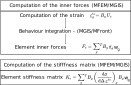
\includegraphics[width=0.6\textwidth]{img/behaviour-integrators.pdf}
\end{center}

\begin{itemize}
\tightlist
\item
  Behaviour integrators are called in the assembly loop over the
  elements for:

  \begin{itemize}
  \tightlist
  \item
    the residual (contribution of the inner forces)
  \item
    the jacobian matrix (i.e.~the tangent stiffness matrix)
  \end{itemize}
\end{itemize}
\end{frame}

\begin{frame}[fragile]{Computation of the inner forces}
\protect\hypertarget{computation-of-the-inner-forces}{}
\begin{Shaded}
\begin{Highlighting}[]
  \KeywordTok{template}\NormalTok{ \textless{}Hypothesis H\textgreater{}}
  \DataTypeTok{void}\NormalTok{ SmallStrainMechanicalBehaviourIntegrator\textless{}H\textgreater{}::updateInnerForces(}
\NormalTok{      mfem::Vector \&Fe,}
      \AttributeTok{const}\NormalTok{ mgis::span\textless{}}\AttributeTok{const}\NormalTok{ real\textgreater{} \&s,}
      \AttributeTok{const}\NormalTok{ mfem::DenseMatrix \&dN,}
      \AttributeTok{const}\NormalTok{ real w,}
      \AttributeTok{const} \DataTypeTok{size\_type}\NormalTok{ ni) }\AttributeTok{const}\NormalTok{ \{}
    \KeywordTok{constexpr} \AttributeTok{const} \KeywordTok{auto}\NormalTok{ icste = }\FloatTok{0.70710678118654752440}\NormalTok{;}
    \KeywordTok{static\_assert}\NormalTok{(H == Hypothesis::TRIDIMENSIONAL, }\StringTok{"unsupported hypothesis"}\NormalTok{);}
    \ControlFlowTok{if} \KeywordTok{constexpr}\NormalTok{ (H == Hypothesis::TRIDIMENSIONAL) \{}
      \AttributeTok{const} \KeywordTok{auto}\NormalTok{ nnodes = dN.NumRows();}
      \AttributeTok{const} \KeywordTok{auto}\NormalTok{ nx = ni;}
      \AttributeTok{const} \KeywordTok{auto}\NormalTok{ ny = ni + nnodes;}
      \AttributeTok{const} \KeywordTok{auto}\NormalTok{ nz = ni + }\DecValTok{2}\NormalTok{ * nnodes;}
\NormalTok{      real B[}\DecValTok{6}\NormalTok{][}\DecValTok{3}\NormalTok{] = \{\{dN(ni, }\DecValTok{0}\NormalTok{), }\DecValTok{0}\NormalTok{, }\DecValTok{0}\NormalTok{\},                          }\CommentTok{//}
\NormalTok{                      \{}\DecValTok{0}\NormalTok{, dN(ni, }\DecValTok{1}\NormalTok{), }\DecValTok{0}\NormalTok{\},                          }\CommentTok{//}
\NormalTok{                      \{}\DecValTok{0}\NormalTok{, }\DecValTok{0}\NormalTok{, dN(ni, }\DecValTok{2}\NormalTok{)\},                          }\CommentTok{//}
\NormalTok{                      \{dN(ni, }\DecValTok{1}\NormalTok{) * icste, dN(ni, }\DecValTok{0}\NormalTok{) * icste, }\DecValTok{0}\NormalTok{\},  }\CommentTok{// xy}
\NormalTok{                      \{dN(ni, }\DecValTok{2}\NormalTok{) * icste, }\DecValTok{0}\NormalTok{, dN(ni, }\DecValTok{0}\NormalTok{) * icste\},  }\CommentTok{// xz}
\NormalTok{                      \{}\DecValTok{0}\NormalTok{, dN(ni, }\DecValTok{2}\NormalTok{) * icste, dN(ni, }\DecValTok{1}\NormalTok{) * icste\}\}; }\CommentTok{// yz}
\NormalTok{      Fe[nx] += w * (B[}\DecValTok{0}\NormalTok{][}\DecValTok{0}\NormalTok{] * s[}\DecValTok{0}\NormalTok{] + B[}\DecValTok{1}\NormalTok{][}\DecValTok{0}\NormalTok{] * s[}\DecValTok{1}\NormalTok{] + B[}\DecValTok{2}\NormalTok{][}\DecValTok{0}\NormalTok{] * s[}\DecValTok{2}\NormalTok{] +}
\NormalTok{                     B[}\DecValTok{3}\NormalTok{][}\DecValTok{0}\NormalTok{] * s[}\DecValTok{3}\NormalTok{] + B[}\DecValTok{4}\NormalTok{][}\DecValTok{0}\NormalTok{] * s[}\DecValTok{4}\NormalTok{] + B[}\DecValTok{5}\NormalTok{][}\DecValTok{0}\NormalTok{] * s[}\DecValTok{5}\NormalTok{]);}
\NormalTok{      Fe[ny] += w * (B[}\DecValTok{0}\NormalTok{][}\DecValTok{1}\NormalTok{] * s[}\DecValTok{0}\NormalTok{] + B[}\DecValTok{1}\NormalTok{][}\DecValTok{1}\NormalTok{] * s[}\DecValTok{1}\NormalTok{] + B[}\DecValTok{2}\NormalTok{][}\DecValTok{1}\NormalTok{] * s[}\DecValTok{2}\NormalTok{] +}
\NormalTok{                     B[}\DecValTok{3}\NormalTok{][}\DecValTok{1}\NormalTok{] * s[}\DecValTok{3}\NormalTok{] + B[}\DecValTok{4}\NormalTok{][}\DecValTok{1}\NormalTok{] * s[}\DecValTok{4}\NormalTok{] + B[}\DecValTok{5}\NormalTok{][}\DecValTok{1}\NormalTok{] * s[}\DecValTok{5}\NormalTok{]);}
\NormalTok{      Fe[nz] += w * (B[}\DecValTok{0}\NormalTok{][}\DecValTok{2}\NormalTok{] * s[}\DecValTok{0}\NormalTok{] + B[}\DecValTok{1}\NormalTok{][}\DecValTok{2}\NormalTok{] * s[}\DecValTok{1}\NormalTok{] + B[}\DecValTok{2}\NormalTok{][}\DecValTok{2}\NormalTok{] * s[}\DecValTok{2}\NormalTok{] +}
\NormalTok{                     B[}\DecValTok{3}\NormalTok{][}\DecValTok{2}\NormalTok{] * s[}\DecValTok{3}\NormalTok{] + B[}\DecValTok{4}\NormalTok{][}\DecValTok{2}\NormalTok{] * s[}\DecValTok{4}\NormalTok{] + B[}\DecValTok{5}\NormalTok{][}\DecValTok{2}\NormalTok{] * s[}\DecValTok{5}\NormalTok{]);}
\NormalTok{    \}}
\NormalTok{  \}  }\CommentTok{// end of updateInnerForces}
\end{Highlighting}
\end{Shaded}

\begin{itemize}
\tightlist
\item
  Note: code from the first versions of \texttt{mfem-mgis}
\item
  The \texttt{B} matrix have numerous null entries.

  \begin{itemize}
  \tightlist
  \item
    The computation of \texttt{F} can easily be optimised.
  \end{itemize}
\end{itemize}
\end{frame}

\begin{frame}[fragile]{Computation of the inner forces (optimized)}
\protect\hypertarget{computation-of-the-inner-forces-optimized}{}
\begin{Shaded}
\begin{Highlighting}[]
  \KeywordTok{template}\NormalTok{ \textless{}Hypothesis H\textgreater{}}
  \DataTypeTok{void}\NormalTok{ SmallStrainMechanicalBehaviourIntegrator\textless{}H\textgreater{}::updateInnerForces(}
\NormalTok{      mfem::Vector \&Fe,}
      \AttributeTok{const}\NormalTok{ mgis::span\textless{}}\AttributeTok{const}\NormalTok{ real\textgreater{} \&s,}
      \AttributeTok{const}\NormalTok{ mfem::DenseMatrix \&dN,}
      \AttributeTok{const}\NormalTok{ real w,}
      \AttributeTok{const} \DataTypeTok{size\_type}\NormalTok{ ni) }\AttributeTok{const}\NormalTok{ \{}
    \KeywordTok{constexpr} \AttributeTok{const} \KeywordTok{auto}\NormalTok{ icste = }\FloatTok{0.70710678118654752440}\NormalTok{;}
    \KeywordTok{static\_assert}\NormalTok{(H == Hypothesis::TRIDIMENSIONAL, }\StringTok{"unsupported hypothesis"}\NormalTok{);}
    \ControlFlowTok{if} \KeywordTok{constexpr}\NormalTok{ (H == Hypothesis::TRIDIMENSIONAL) \{}
      \AttributeTok{const} \KeywordTok{auto}\NormalTok{ nnodes = dN.NumRows();}
      \AttributeTok{const} \KeywordTok{auto}\NormalTok{ nx = ni;}
      \AttributeTok{const} \KeywordTok{auto}\NormalTok{ ny = ni + nnodes;}
      \AttributeTok{const} \KeywordTok{auto}\NormalTok{ nz = ni + }\DecValTok{2}\NormalTok{ * nnodes;}
\NormalTok{      real B[}\DecValTok{6}\NormalTok{][}\DecValTok{3}\NormalTok{] = \{\{dN(ni, }\DecValTok{0}\NormalTok{), }\DecValTok{0}\NormalTok{, }\DecValTok{0}\NormalTok{\},                          }\CommentTok{//}
\NormalTok{                      \{}\DecValTok{0}\NormalTok{, dN(ni, }\DecValTok{1}\NormalTok{), }\DecValTok{0}\NormalTok{\},                          }\CommentTok{//}
\NormalTok{                      \{}\DecValTok{0}\NormalTok{, }\DecValTok{0}\NormalTok{, dN(ni, }\DecValTok{2}\NormalTok{)\},                          }\CommentTok{//}
\NormalTok{                      \{dN(ni, }\DecValTok{1}\NormalTok{) * icste, dN(ni, }\DecValTok{0}\NormalTok{) * icste, }\DecValTok{0}\NormalTok{\},  }\CommentTok{// xy}
\NormalTok{                      \{dN(ni, }\DecValTok{2}\NormalTok{) * icste, }\DecValTok{0}\NormalTok{, dN(ni, }\DecValTok{0}\NormalTok{) * icste\},  }\CommentTok{// xz}
\NormalTok{                      \{}\DecValTok{0}\NormalTok{, dN(ni, }\DecValTok{2}\NormalTok{) * icste, dN(ni, }\DecValTok{1}\NormalTok{) * icste\}\}; }\CommentTok{// yz}
\NormalTok{      Fe[nx] += w * (B[}\DecValTok{0}\NormalTok{][}\DecValTok{0}\NormalTok{] * s[}\DecValTok{0}\NormalTok{] + B[}\DecValTok{3}\NormalTok{][}\DecValTok{0}\NormalTok{] * s[}\DecValTok{3}\NormalTok{] + B[}\DecValTok{4}\NormalTok{][}\DecValTok{0}\NormalTok{] * s[}\DecValTok{4}\NormalTok{]);}
\NormalTok{      Fe[ny] += w * (B[}\DecValTok{1}\NormalTok{][}\DecValTok{1}\NormalTok{] * s[}\DecValTok{1}\NormalTok{] + B[}\DecValTok{3}\NormalTok{][}\DecValTok{1}\NormalTok{] * s[}\DecValTok{3}\NormalTok{] + B[}\DecValTok{5}\NormalTok{][}\DecValTok{1}\NormalTok{] * s[}\DecValTok{5}\NormalTok{]);}
\NormalTok{      Fe[nz] += w * (B[}\DecValTok{2}\NormalTok{][}\DecValTok{2}\NormalTok{] * s[}\DecValTok{2}\NormalTok{] + B[}\DecValTok{4}\NormalTok{][}\DecValTok{2}\NormalTok{] * s[}\DecValTok{4}\NormalTok{] + B[}\DecValTok{5}\NormalTok{][}\DecValTok{2}\NormalTok{] * s[}\DecValTok{5}\NormalTok{]);}
\NormalTok{    \}}
\NormalTok{  \}  }\CommentTok{// end of updateInnerForces}
\end{Highlighting}
\end{Shaded}

\begin{itemize}
\tightlist
\item
  Note: code from the first versions of \texttt{mfem-mgis}
\end{itemize}
\end{frame}

\begin{frame}{Code generation}
\protect\hypertarget{code-generation}{}
\begin{itemize}
\tightlist
\item
  Behaviour integrators are meant to:

  \begin{itemize}
  \tightlist
  \item
    Compute the gradients from unknowns (using the \(B\) matrix).
  \item
    Handle the state variables.
  \item
    Call the behaviour integration.
  \item
    Compute the inner forces from the thermodynamic forces.
  \item
    Compute the stiffness matrix from the consistent tangent operator
    blocks.
  \end{itemize}
\end{itemize}

\vspace*{1mm}

\begin{itemize}
\tightlist
\item
  All those steps depends on:

  \begin{itemize}
  \tightlist
  \item
    The type of problem described (mechanics, heat transfer).
  \item
    The symmetry of the material (isotropic or orthotropic).
  \item
    The modelling hypotheses (\(3D\), plane strain, plane stress,
    axisymmetry, etc\ldots).
  \end{itemize}
\end{itemize}

\vspace*{1mm}

\begin{itemize}
\tightlist
\item
  The writting of behaviour integrators is tedious and error-prone\\
  and shall be done with care (see example)

  \begin{itemize}
  \tightlist
  \item
    However, specific behaviour integrators gives access to pieces of
    physics.
  \item
    Code generation to the rescue !
  \end{itemize}
\end{itemize}
\end{frame}

\begin{frame}[fragile]{The \texttt{behaviour-integrator} code generator}
\protect\hypertarget{the-behaviour-integrator-code-generator}{}
\begin{itemize}
\tightlist
\item
  Aim of this code-generator

  \begin{itemize}
  \tightlist
  \item
    Generate behaviour integrators
  \item
    Code factorisation
  \item
    Avoid coding errors due to tedious formula
  \end{itemize}
\end{itemize}

\vspace*{1mm}

\begin{itemize}
\tightlist
\item
  Machinery

  \begin{itemize}
  \tightlist
  \item
    Based on the \texttt{GiNaC} for symbolic computations in
    \texttt{C++}
  \item
    Current scope: isotropic and orthotropic, small and finite strain
    behaviours in plane strain, plane stress and tridimensional.
  \end{itemize}
\end{itemize}

\vspace*{1mm}

\begin{itemize}
\tightlist
\item
  Extensions (to come)

  \begin{itemize}
  \tightlist
  \item
    Support of axisymmetry
  \item
    Non linear heat transfer, non linear diffusion.
  \item
    Can be extended to other non-linear models, wide range of phenomena.
  \end{itemize}
\end{itemize}
\end{frame}





\section{Feed-backs on some limitations of {\tt MFEM}}
\Intercalaire{Feed-backs on some limitations of {\tt MFEM}}

\Titre{Handling failures of the behaviour integration}
\frame{
}

\Titre{Imposition of Dirichlet boundary conditions}
\frame{
  \begin{center}
    \includegraphics[width=0.75\textwidth]{img/DiricheltBoundaryConditionIssue.pdf}
  \end{center}
}

\section{Conclusions and perspectives}
\Intercalaire{Conclusions and perspectives}

\Titre{Conclusions and perspectives}
\frame{}

\end{document}
